\documentclass[12pt,a4paper]{report}

%%%%%%%%%%%%%%%%%%%%%%%%%%%%%%%%%%%%%%%%
%           Liste des packages         %
%%%%%%%%%%%%%%%%%%%%%%%%%%%%%%%%%%%%%%%%
%% Faux texte
\usepackage{blindtext}

%%%%%%%%%%%%%%%%%%%%%%%%%%%%%%%%%%%%%%%%%%%%%%%%%%%%%%%%%%%%%%%%%%%%%
%% Réglage des fontes et typo    
\usepackage[utf8]{inputenc}

\usepackage[top=2.5cm, bottom=2cm, left=3cm, right=2.5cm, headheight=15pt]{geometry} 

\usepackage[frenchb]{babel}
\usepackage{lmodern} 					% Pour changer le pack de police.
\usepackage[upright]{fourier}			% Police tsara
\usepackage{pdfpages}					% Inclure pdf
\usepackage{pdflscape}					% Permet d'utiliser des pages au format paysage

\setlength{\parindent}{0pt} 			% supprime l'indentation
\sloppy									%	
\hyphenpenalty 10000					% empeche la coupure des mots

\usepackage{moreverb} % Code source avec tabulation
%%%%%%%%%%%%%%%%%%%%%%%%%%%%%%%%%%%%%%%%%%%%%%%%%%%%%%%%%%%%%%%%%%%%%
% ABSTRACT


%%%%%%%%%%%%%%%%%%%%%%%%%%%%%%%%%%%%%%%%%%%%%%%%%%%%%%%%%%%%%%%%%%%%%
% En-tête et pied de pages
\usepackage{fancyhdr}

\pagestyle{fancy}
\lhead{}
\chead{}
\rhead{Conception et  réalisation du logiciel de gestion de la Polyclinique universitaire NEXT}
\lfoot{}
\cfoot{\thepage}
\rfoot{} 	
	
%%%%%%%%%%%%%%%%%%%%%%%%%%%%%%%%%%%%%%%%%%%%%%%%%%%%%%%%%%%%%%%%%%%%%
% Images 
\usepackage{graphicx} 		% Images
\usepackage{wrapfig} 		% Images

%%%%%%%%%%%%%%%%%%%%%%%%%%%%%%%%%%%%%%%%%%%%%%%%%%%%%%%%%%%%%%%%%%%%%
% Tableaux
\usepackage{multirow}
\usepackage{booktabs}
\usepackage{colortbl}
\usepackage{tabularx}
\usepackage{multirow}
\usepackage{threeparttable}

\addto\captionsfrench{\def\tablename{{\textsc{Tableau}}}}	% Renome 'table' en 'tableau'

\usepackage{supertabular}

\definecolor{grisclair}{gray}{0.8} % Définition d'une couleur gris

%%%%%%%%%%%%%%%%%%%%%%%%%%%%%%%%%%%%%%%%%%%%%%%%%%%%%%%%%%%%%%%%%%%%%
% Math
\usepackage{amsmath} 
\usepackage{amssymb} 
\usepackage{mathrsfs}
\usepackage{amsthm}
	
%%%%%%%%%%%%%%%%%%%%%%%%%%%%%%%%%%%%%%%%%%%%%%%%%%%%%%%%%%%%%%%%%%%%%   
% Table des matières
\usepackage[francais]{minitoc}		% Mini table des matières, en français
	\setcounter{minitocdepth}{2}	% Mini-toc détaillée (sections/sous-sections)
	
% Mettre Chapitre 1. "nom du chapitre" dans le table of contents
\usepackage{titletoc}
\titlecontents*{chapter} % <section type>
	[0pt] % <left>
	{\addvspace{1em}} %
	{\bfseries\chaptername\ \thecontentslabel\quad}% <numbered-entry-format}
	{} % <numbereless-entry-format>
	{\bfseries\hfill\contentspage} % <filler-page-format>

%%%%%%%%%%%%%%%%%%%%%%%%%%%%%%%%%%%%%%%%%%%%%%%%%%%%%%%%%%%%%%%%%%%%%
% Glossaire
\usepackage{glossaries}
\newglossary[nlg]{notation}{not}{ntn}{Notation}
\makeglossaries

\usepackage{hyphenat}
%\setacronymstyle{long-short}

%%%%%%%%%%%%%%%%%%%%%%%%%%%%%%%%%%%%%%%%%%%%%%%%%%%%%%%%%%%%%%%%%%%%%
% Biblio                        
%\usepackage{natbib}

%%%%%%%%%%%%%%%%%%%%%%%%%%%%%%%%%%%%%%%%%%%%%%%%%%%%%%%%%%%%%%%%%%%%%
%% Navigation dans le document   
\usepackage[pdftex,pdfborder={0 0 0},
			colorlinks=true,
			linkcolor=black,
			citecolor=black,
			pagebackref=false,
			]{hyperref} %Créera automatiquement les liens internes au PDF
			
%%%%%%%%%%%%%%%%%%%%%%%%%%%%%%%%%%%%%%%%%%%%%%%%%%%%%%%%%%%%%%%%%%%%%
%% Compilation
\usepackage{silence}
%
%% Virer les erreur dues à minitoc
\WarningFilter{minitoc(hints)}{W0023}
\WarningFilter{minitoc(hints)}{W0024}
\WarningFilter{minitoc(hints)}{W0028}
\WarningFilter{minitoc(hints)}{W0030}			 	% Liste des packages et de leurs options

\usepackage{supertabular}

%%%%%%%%%%%%%%%%%%%%%%%%%%%%%%%%%%%%%%%%%%%%%
%		LISTE DES ACRONYMES
%%%%%%%%%%%%%%%%%%%%%%%%%%%%%%%%%%%%%%%%%%%%%
\newacronym{espa}{ESPA}{Ecole Supérieure Polytechnique d'Antsiranana}
\newacronym{saas}{SaaS}{Software as a Service}
\newacronym{sla}{SLA}{Service-Level Agreement}
\newacronym{soa}{SOA}{Service Oriented Architecture}
\newacronym{api}{API}{Interface de Programmation Applicative}
\newacronym{god}{GoD}{Gaming on Demand}
\newacronym{lmd}{LMD}{Licence-Master-Doctorat}
\newacronym{ue}{UE}{Unité d'Enseignement}
\newacronym{ec}{EC}{Elément Constitutif}
\newacronym{sis}{SIS}{Student Information Systems}
\newacronym{crm}{CRM}{Customer Relationship Management}
\newacronym{grc}{GRC}{Gestion de la Relation Client}
\newacronym{sgbd}{SGBD}{Système de Gestion de Base de Données}
\newacronym{jee}{JEE}{Java Etreprise Edition}
\newacronym{html}{HTML}{Hypertext Markup Language}
\newacronym{css}{CSS}{Cascading Style Sheets}
\newacronym{mvc}{MVC}{Model View Controller}
\newacronym{jsf}{JSF}{Java Server Faces}
\newacronym{jsp}{JSP}{Java Server Pages}
\newacronym{jstl}{JSTL}{JavaServer Pages Standard Tag Library}
\newacronym{rh}{RH}{Ressources Humaines}
\newacronym{grh}{GRH}{Gestion des Ressources Humaines}
\newacronym{bdd}{BDD}{Base de Données}
\newacronym{uml}{UML}{Unified Modeling Language}
\newacronym{cv}{CV}{Curriculum Vitæ}
\newacronym{mcd}{MCD}{Modèle Conceptuel des Données}
\newacronym{mld}{MLD}{Modèle Logique de Données}

\newacronym{json}{JSON}{JavaScript Object Notation}
\newacronym{spa}{SPA}{Single-Page Application}
\newacronym{adsl}{ADSL}{Asymmetric Digital Subscriber Line}



%%%%%%%%%%%%%%%%%%%%%%%%%%%%%%%%%%%%%%%%%%%%%
%		LISTE DES GLOSSAIRES
%%%%%%%%%%%%%%%%%%%%%%%%%%%%%%%%%%%%%%%%%%%%%
\newglossaryentry{multiTenant}{
	type=notation,
	name={Multi-tenant},
	description={En informatique, multi-tenant, ou multi-entité désigne un principe d'architecture logicielle permettant à un logiciel de servir plusieurs organisations clientes à partir d'une seule installation},
}
\newglossaryentry{cloudComputing}{
	type=notation,
	name={Cloud computing},
	description={Le cloud computing, ou l'informatique en nuage ou nuagique ou encore l'infonuagique, est l'exploitation de la puissance de calcul ou de stockage de serveurs informatiques distants par l'intermédiaire d'un réseau, généralement internet},
	sort={N}%
}
\newglossaryentry{gamingOnDemand}{
	type=notation,
	name={Gaming on Demand},
	description={Jeu à la demande en français, est une technologie similaire à la vidéo à la demande permettant de jouer normalement à des jeux vidéo sur son écran d'ordinateur ou sa télévision alors que celui-ci tourne sur des serveurs à distance qui renvoient la vidéo de ce qui a été joué en lecture en continu (communément appelé streaming)},
	sort={N}%
}
\newglossaryentry{middleware}{
	type=notation,
	name={Middleware},
	description={Ou intergiciel est un logiciel tiers qui crée un réseau d'échange d'informations entre différentes applications informatiques.},
	sort={N}%
}
\glsaddall % print all gls

\renewcommand{\thesubsubsection}{\alph{subsubsection})}

\begin{document}
	
\includepdf{Couverture/Couverture.pdf} 
		
	
\includepdf{PageDeGarde/PageDeGarde.pdf} 
	
	
\includepdf[pages=1-2]{CahierDeCharge/CahierDeCharge.pdf}
		
	\pagenumbering{roman} 			% Page en chiffre romain
		
	\dominitoc						% Génération des mini-toc	
		
	%%%%%%%%%%%%%%%%%%%%%%%%%%%%%%%%%%%%%%%%%%%%%%%%%%%%%%%%%%%%%%%%%%%%%%%%%%%%%%%%%%%%%%%%%%%%%
%%									   Remerciement	    								 %%
%%%%%%%%%%%%%%%%%%%%%%%%%%%%%%%%%%%%%%%%%%%%%%%%%%%%%%%%%%%%%%%%%%%%%%%%%%%%%%%%%%%%%%%%%%%%%
\chapter*{Remerciements}
\addstarredchapter{Remerciements}

%%%%%%%%%%%%%%%%%%%%%%%%%%%%%%%%%%%%%
%%  redéfinition de l'interligne   %%
%%%%%%%%%%%%%%%%%%%%%%%%%%%%%%%%%%%%%

{\setlength{\baselineskip}{1.5\baselineskip}

%%%%%%%%%%%%%%%%%%%%%%%%%%%%%%%%%%%%%

En préambule de ce travail, j'aimerai exprimer, par ces quelques lignes de remerciements,
mes gratitudes envers tous ceux en qui, par leur présence, leur soutien, leur disponibilité
et leurs conseils j'ai trouvé courage pour réaliser ce travail.
\bigskip

En premier lieu, j'adresse mes respectueuses considérations à mon encadreur
professionnel : Dr. ANDRIAMIHARINJAKA Hasina, qui a été l'esprit pensant donnant
naissance à ce sujet et qui m'a dirigée par ses précieux conseils tout en me laissant la
liberté d'initiative pour la conception de la plateforme. A mes encadreurs qui sont M.
ANDRINIRINIAIMALAZA Fanambinantsoa Philibert et M. RAMANAN'HAJA Hery Tina,
pour avoir dirigés ce travail, pour leurs soucient et aussi pour leurs aides et leurs
orientations qui m'ont permis de réaliser ce travail dans les meilleures conditions.
\bigskip

J'adresse mes remerciements anticipés et mes honorables considérations également aux
membres de Jury qui vont évaluer et porter leur jugement à ce travail, aussi en enrichir le
contenu par leurs précieuses propositions.
\bigskip

Je dois reconnaissance également à l'ensemble du corps enseignant de la mention STIC
de leESPA (Ecole Supérieure Polytechnique d'Antsiranana).
\bigskip

Une mention particulière à ma famille, pour leurs soutiens et leurs attentions sans faille,
dont les encouragements et l'amour.
\bigskip

Bref, tout ceux qui ont contribué de près ou de loin à l'accomplissement de ce travail.

\null\hfill RATSIZAFY Heriniaina Midonique

%%%%%%%%%%%%%%%%%%%%%%%%%%%%%%%%%%%%%%
%% fin redéfinition de l'interligne %%
%%%%%%%%%%%%%%%%%%%%%%%%%%%%%%%%%%%%%%

\par}

%%%%%%%%%%%%%%%%%%%%%%%%%%%%%%%%%%%%%

	
	
	
	% Sommaire
	\setcounter{tocdepth}{1} % Pas besoin de trop détailler le sommaire (chapitres/sections)	
	\tableofcontents
	\addstarredchapter{Table des matières}
	\cleardoublepage
	
	% Liste des figures
	\renewcommand{\listfigurename}{Liste des figures}
	\listoffigures
	\addstarredchapter{Liste des figures}
	
	% Liste des tableaux	
	\listoftables
	\addstarredchapter{Liste des tableaux}
	\newpage
	
	% Liste des acronyme
	\printglossary[title={Liste des acronymes}, toctitle={Liste des acronymes},nonumberlist]
	\addstarredchapter{Liste des acronymes}
	
	% Glossaires
	\printglossary[type=notation,title={Glossaire}, toctitle={Glossaire},nonumberlist]	
	\addstarredchapter{Glossaire}
	
	%%%%%%%%%%%%%%%%%%%%%%%%%%%%%%%%%%%%%		
	% 		Contenu du document			%
	%%%%%%%%%%%%%%%%%%%%%%%%%%%%%%%%%%%%%
	
	%%%%%%%%%%%%%%%%%%%%%%%%%%%%%%%%%%%%%
	%%  redéfinition de l'interligne   %%
	%%%%%%%%%%%%%%%%%%%%%%%%%%%%%%%%%%%%%
	\newpage
	\pagenumbering{arabic} % Page en chiffre arabe 1, 2, 3
	
	{\setlength{\baselineskip}{1.5\baselineskip}
		
		%%%%%%%%%%%%%%%%%%%%%%%%%%%%%%%%%%%%%
		
		%%%%%%%%%%%%%%%%%%%%%%%%%%%%%%%%%%%%%%%%%%%%%%%%%%%%%%%%%%%%%%%%%%%%%%%%%%%%%%%%%%%%%%%%%%%%%
%%									   Introduction		    							   %%
%%%%%%%%%%%%%%%%%%%%%%%%%%%%%%%%%%%%%%%%%%%%%%%%%%%%%%%%%%%%%%%%%%%%%%%%%%%%%%%%%%%%%%%%%%%%%
\chapter*{Introduction générale}
\addstarredchapter{Introduction générale}
Polyclinique Next dispose de différent branche qui offre de variété de service. que ce soit  patient, personnel ou d'autre entité toute cette personnage engendre de grande quantité d'information. Qui nécessite d'être traité et organisé .  la présence de grand quantité d'information qui s'échange constamment au sein de chaque service s'avère très difficile à manoeuvrer sans la présence d'un logiciel spécifique pour automatiser certaine fonctionnalité. 
  		Grâce au partenariat avec la polyclinique Next et l'école supérieur polytechnique, moi, les encadreur,et les gent du polyclinique ont mis d'accord pour oeuvrer à la conception et réalisation d'un logiciel de gestion qui a pur but d'automatiser la fonctionnalité précédemment évoque dans le cahier de charge suivante.


		%%%%%%%%%%%%%%%%%%%%%%%%%%%%%%%%%%%%%%%%%%%%%%%%%%%%%%%%%%%%%%%%%%%%%%%%%%%%%%%%%%%%%%%%%%%%%
%%									   Chapitre 1	    								   %%
%%%%%%%%%%%%%%%%%%%%%%%%%%%%%%%%%%%%%%%%%%%%%%%%%%%%%%%%%%%%%%%%%%%%%%%%%%%%%%%%%%%%%%%%%%%%%
\chapter{GENERALITE}
\minitoc
\newpage
%%%%%%%%%%%%%%%%%%%%%%%%%%%%%%%%%%%%%
\section{Introduction}

	\section{Bref Historique du polyclinique Universitair NEXT}
  	
  	La NEXT onlus a été fondée en 1998 par un chercheur scientifique, Luigi BELLINI, qui, à la
  	suite d'un voyage à Madagascar, profondément touché par les terribles conditions de vie de
  	la majorité (80\%) des personnes vivant avec moins d'un dollar par jour, a décidé
  	d'entreprendre une action pour aider ces gens, en consacrant toutes ses énergies et
  	ressources à ce but.
  	\medskip
  	
  	Le travail d'organisation et d'assistance s'est progressivement développé avec une
  	particulière attention dans le domaine de la santé dans le Nord de Madagascar, où ont été
  	accomplies des oeuvres importantes qui interagissent avec le système actuel de la Santé
  	Publique
  	\medskip
  	
  	L'activité de la NEXT, développée au début avec ses propres moyens financiers et sans le
  	soutien d'organismes extérieurs, a été reconnue par l'État Italien, qui, en Octobre 2006, lui a
  	accordé le statut juridique d'ONG (Organisation Non Gouvernementale).
  	\medskip
  	
  	Le professeur Luigi BELLINI a progressivement abandonné ses activités en Italie, ses
  	travaux de recherche à l'Université et professionnel, même sa collaboration scientifique avec
  	l'Agence spatiale européenne. Il a décidé de réaliser un centre de diagnostic médical à
  	Madagascar, dénommé « Le Samaritain ». Le centre, d'une superficie de 3 000 m2,
  	comprenant des laboratoires de radiologie et d'échographie, a débuté ses activités, en 2006.
  	Il est doté d'équipements modernes de niveau européen.
  	\medskip
  	
  	En constatant que le centre de diagnostic à lui seul ne suffit pas, l'ONG a mis sur les rails la
  	première clinique de maternité et de chirurgie dans le Nord. Une grande réalisation, unique à
  	Madagascar. Les travaux de construction ont débuté en 2009 : ce fut les premières
  	fondations de la Polyclinique universitaire NEXT.
  	
  	\medskip
  	
  
		
		\section{Localisation et  information sur le complex hospitalier}
		
		
		\subsection{localisation}
		Le Centre "Le Samaritain" ainsi que la Clinique de Maternité et Chirurgie se trouvent dans la
		région DIANA, située au Nord de Madagascar.
		(Pour arriver au complexe sanitaire il faut s'engager sur la route nationale 6 (RN6) et
		procéder 200 m avant de tourner à gauche vers « Rue de la Fraternité ».)
		
		\subsection{ Information concernant le complexe hospirtalier}
		
		L'objectif de la NEXT était d'assurer l'assistance médicale aux gens de la Région
		d'Antsiranana et de toutes les Provinces du Nord de Madagascar par la construction et
		l'équipement d'une Clinique, située à côté du Centre de Diagnostic Médical "Le Samaritain".
		Cette nouvelle structure à trois étages abritera les départements de maternité, chirurgie
		générale et médecine et sera équipée de :
		
		\begin{itemize}
			\item une salle opératoire principale

			\item une salle opératoire d'urgence ou secondaire

			\item une salle d'accouchement
			
			\item une salle de stérilisation

			\item une salle postopératoire
			
			\item un centre d'hémodialyse
			
			\item  un service d'urgences.
		\end{itemize}
		
		
		\subsection{Plan hospitalier}
		L'établissement de santé est reparti comme suit:
	
		\medskip
		\begin{tabular}{|c|c|c|}
		\hline  REZ-DE-CHAUSSÉE & 1ER ETAGE : & 2EME ETAGE \\ 
		\hline Triage-urgence & Bloc opératoire & Médecine \\ 
		 Hemodialyse & Chirurgie  & Pharmacie \\ 
		 Direction-administration & Gynéco-obstétrique & Salle de classe \\ 
		  & Maternité & Présidence \\ 
		  & Salle d'accouchement &  \\ 
		\hline 
		\end{tabular} 
		\medskip
		
		\section{Généralité sur le web}
		
		\section{Choix de la technologie utilisé}
		
	
		%%%%%%%%%%%%%%%%%%%%%%%%%%%%%%%%%%%%%%%%%%%%%%%%%%%%%%%%%%%%%%%%%%%%%%%%%%%%%%%%%%%%%%%%%%%%%
%%									   Chapitre 2	    								 %%
%%%%%%%%%%%%%%%%%%%%%%%%%%%%%%%%%%%%%%%%%%%%%%%%%%%%%%%%%%%%%%%%%%%%%%%%%%%%%%%%%%%%%%%%%%%%%
\chapter{Modélisation statique et dynamique du système}
\minitoc
\newpage
%%%%%%%%%%%%%%%%%%%%%%%%%%%%%%%%%%%%%
\section{Introduction}
Tous les programmes informatiques n’ont pas été construits à l’aveuglette par les
programmeurs, même les plus petits ont fait l’objet de quelques réflexions. Pour notre cas,
quelques réflexions ne suffisent pas, il en faut beaucoup. Mais on peut facilement se perdre
dans ces réflexions si on n’a pas de méthodes et un langage de modélisation bien adaptée. Nous construisons des modèles de systèmes complexes parce nous sommes incapables d'appréhender ces systèmes dans leur entièreté.
 Mais c'est quoi vraiment  un modèle?
\medskip
	  Un modèle est une simplification de
	  la réalité. la modélisation permet alors de maitriser
	  la complexité du système étudié,
	  car chaque modèle donne accès à
	  une représentation abstraite de
	  différents aspects du système.
	modéliser un système   consiste à créer une représentation schématique simplifié d'un problème. Le but est de:
	\begin{itemize}
\item Nous aider à visualiser le système tel qu'il est ou tel qu'il devrait être.
\item Spécifier la structure et le comportement d'un système
\item Avoir un "patron" pour guider la construction du système.
\item Documenter les décisions qui ont été prises
	\end{itemize}
	

	
	% %eventuellement uml definition les diagrame  presentation merise pour la base de donne uml pour la modeleisation
	
	
	
	
	
	
	
	
	
	
	
	
	
	
	
	
	
	
	
	
	
	
	
	
	
	
	\newpage
	\section{Analyse de fonctionnement de l'hôpital}
	Pour se lancer dans la modélisation, on a besoin des information concernant cette établissement sanitaire pour comprendre le mécanisme qui y se trouve.
	De façon générale, le fonctionnement de l'hôpital repose sur l'ordonnancement des
	branches ci dessous.
	
	\subsection{L'accueil }
	Un nouvel arrivant dans le centre hospitalier doit impérativement se présenter à l'accueil.
	De là, le responsable enregistre les renseignements de base du nouveau malade, à
	savoir :
	La date d'entrée, le nom Prénom, le sexe, l'age, l'adresse, le téléphone, le médecin traitant, la famille ou personne externe,  la profession et l'unité d'admission.
	 Sur l'unité d'admission, ceci est à propos du département dans lequel le patient va être orienté
	Il est à noter que les renseignements sus enregistrés, feront l'objet d'une fiche qui
	sera remplie au fur et à mesure du traitement du patient concerné, une fois admis
	dans l'unité d'admission
	
	\medskip
	
	Quand un malade doit être hospitalisé, c'est également à l'accueil que cet évènement
	doit être pris en compte. En effet, le responsable enregistre :
	
	Le numéro du patient (entre autre, son dossier médical), la chambre le lit et la catégorie de la chambre
	
	\medskip
	Comme le rôle de l'accueil se repose surtout sur l'enregistrement du mouvement de la	population hospitalière, à la sortie d'un patient, un personnel de l'accueil enregistre la	sortie, avec les attributs suivants :
	le numéro de patient	le nom et prénom, l'état de sortie (mort, guérison, amélioration, statu-quo), la décision de sortie (de l'hôpital ou volontaire)




\subsection{Les départements d'admission}

A La polyclinique Universitaire NEXT, on retrouve les départements suivants :

la maternité, chirurgie,bloc, opératoire,        néphrologie,  pédiatrie, gynécologie, mise en observation.

Une fois que le patient est orienté vers son unité d'admission, sa fiche sera modifiée, en
rapport avec son suivi médical.


\subsection{L'administration}

Toutes les prestations effectuées par le patient sont notées et enregistrées par un
responsable de administration.


\subsection{La caisse}
La caisse est chargée du service facturation. Quand un patient va passer au paiement, il se
présente à la caisse. Le caissier consulte les prestations saisies par l'administration.
Son rôle vise également à l'évaluation et l'exploitation d'un certain nombre d'informations
et de statistiques, liées à la comptabilité des prestations.

\subsection{La direction}
La direction a dans ses attributs, la gestion des utilisateurs, la diffusion
d'informations/messages au personnel.

\subsection{La médecine}

La section médecine est dédiée aux médecins, plutôt dans le sens de prescription. Quand un
patient se présente alors au cabinet, le médecin lui prescrit une ordonnance









	\newpage
	
	
	
	
	
	
	
	
	
	
	
	\section{Diagrame de cas d'utilisation}
	
	\subsection{Diagramme de cas d'utilisation générale du systéme}
	\begin{figure}[h]
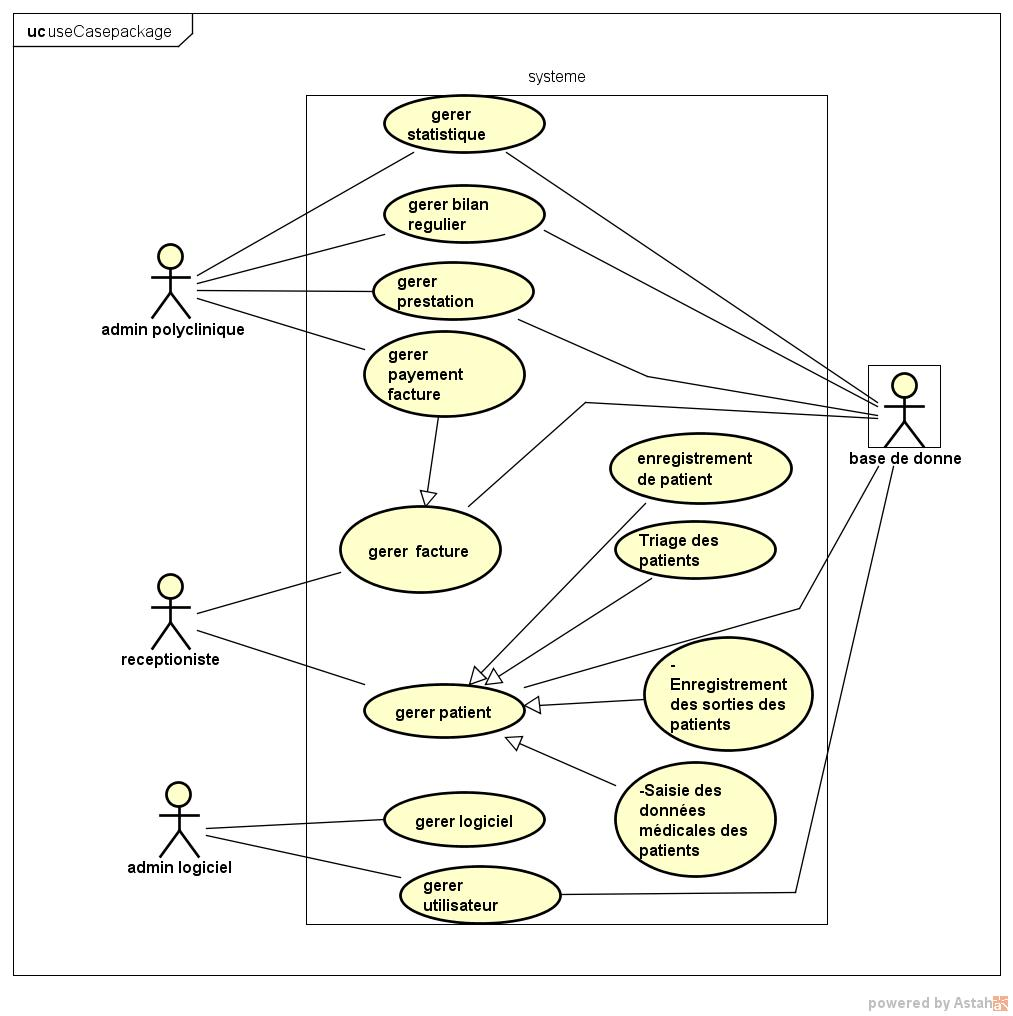
\includegraphics[scale=0.5]{Chapitre2/images/mainUseCaseDiagramme.jpg}
\caption{Diagramme de cas d'utilisation générale du systéme}
	\end{figure}
	
\newpage

	\subsection{Diagramme de cas d'utilisation réceptionniste }
	  
	  \begin{figure}[h]
	  \centering
	   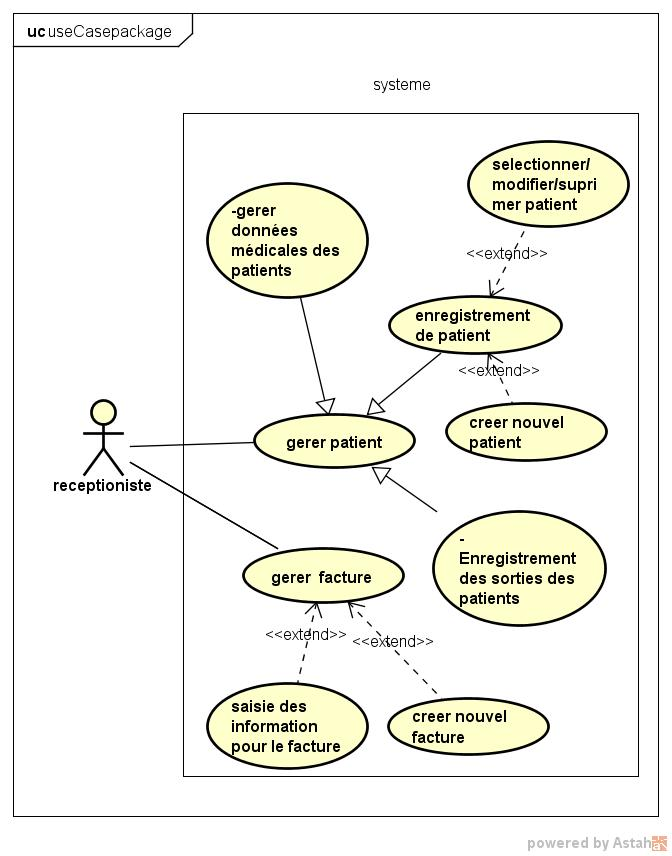
\includegraphics[scale=0.5]{Chapitre2/images/ucdreceptioniste}
	    \caption{Diagramme de cas d'utilisation réceptionniste}
	  \end{figure}
	 
\newpage

	\subsection{Diagramme de cas d'utilisation administrateur polyclinique }
	  
	  \begin{figure}[h]
	  \centering
	  
	   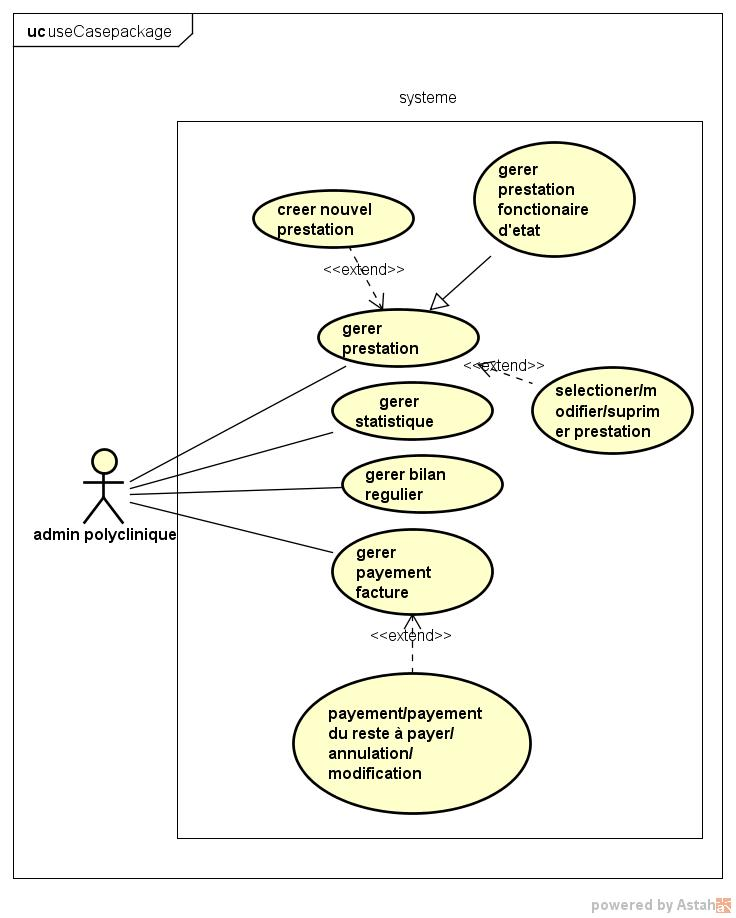
\includegraphics[scale=0.5]{Chapitre2/images/ucdadminPolyclinique.jpg}
	    \caption{Diagramme de cas d'utilisation administrateur polyclinique }
	  \end{figure}
	 
\newpage

	\subsection{Diagramme de cas d'utilisation admin logiciel}
	  
	  \begin{figure}[h]
	  \centering
	   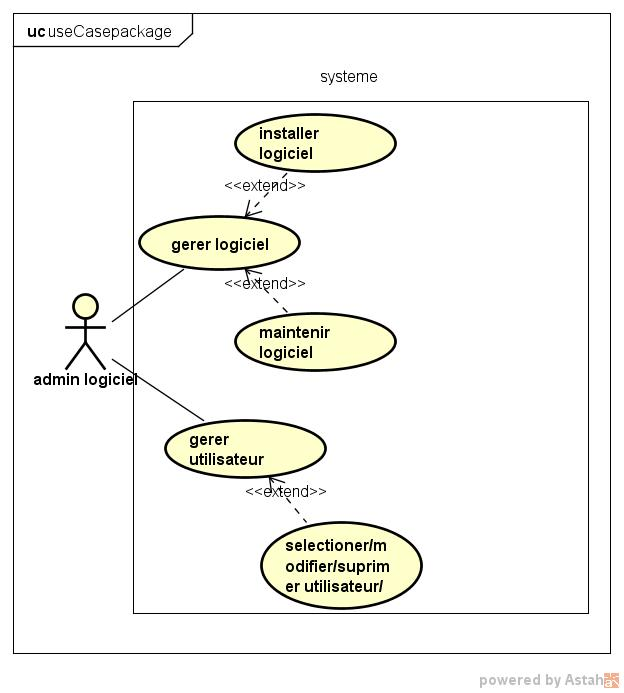
\includegraphics[scale=0.6]{Chapitre2/images/ucdadminlogiciel}
	    \caption{Diagramme de cas d'utilisation administrateur logiciel}
	  \end{figure}
	 
	  \newpage
	  
	  \section{diagramme de séquence}
	  
	  \subsection{Diagrame de sequence gestion patient}
	  \begin{figure}[h]
	  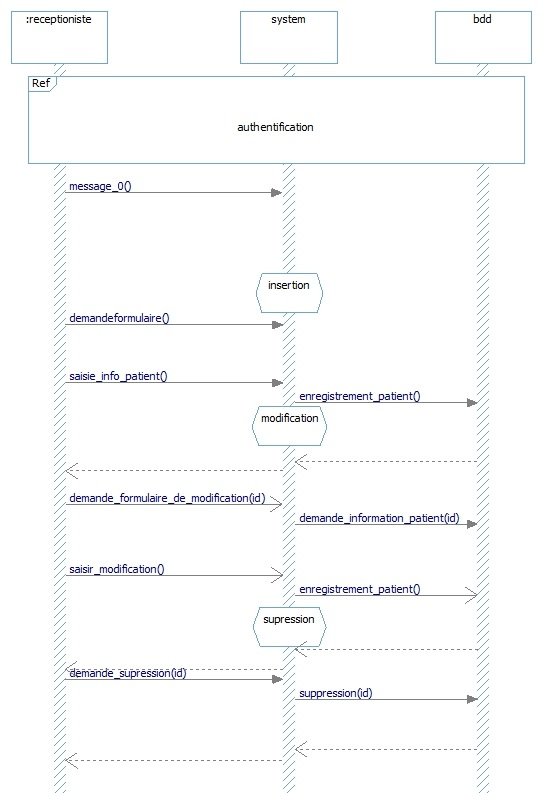
\includegraphics[scale=0.9]{Chapitre2/images/sd_gererpatient}
\caption{Diagramme de  séquence gestion patient}
	  \end{figure}
	  
	  \newpage
	  
	  \subsection{Diagramme de séquence gestion facturation}
	  
	  \section{Diagramme de classe de l'application}
	  
	  \begin{figure}[h]
	  	  \includegraphics[scale=0.75]{Chapitre2/images/classDiagramme}
	  \caption{Diagramme de classe de l'application}
	  	  \end{figure}
	  
	  
	 
	  
	  
	  
	  	
		%%%%%%%%%%%%%%%%%%%%%%%%%%%%%%%%%%%%%%%%%%%%%%%%%%%%%%%%%%%%%%%%%%%%%%%%%%%%%%%%%%%%%%%%%%%%%
%%									   Chapitre 3	    								 %%
%%%%%%%%%%%%%%%%%%%%%%%%%%%%%%%%%%%%%%%%%%%%%%%%%%%%%%%%%%%%%%%%%%%%%%%%%%%%%%%%%%%%%%%%%%%%%
 \chapter{Programmation et réalisation du logiciel}
\minitoc
\newpage
%%%%%%%%%%%%%%%%%%%%%%%%%%%%%%%%%%%%%
\section{Introduction}
	  La réalisation et le codage de l'application est une étape cruciale et inévitable,  dans le développement de l'application, l'application ne se construit tout seul après la modélisation, pour que l'application ne soit pas devenir une simple rêve il faut le produire.
	  \medskip
	  Nous avons utilisé laravel pour le codage.
	  
	  
	  \section{Le framwork Laravel}
	  
	  Les applications Laravel sont installées et gérées avec Composer , un gestionnaire de
	  dépendance PHP. Il existe deux manières de créer une nouvelle application Laravel.
	  
	 Sur le terminal:
	  composer create-project laravel/laravel [foldername]
<<<<<<< HEAD
	%	%%%%%%%%%%%%%%%%%%%%%%%%%%%%%%%%%%%%%%%%%%%%%%%%%%%%%%%%%%%%%%%%%%%%%%%%%%%%%%%%%%%%%%%%%%%%%
%%									   Chapitre 4	    								 %%
%%%%%%%%%%%%%%%%%%%%%%%%%%%%%%%%%%%%%%%%%%%%%%%%%%%%%%%%%%%%%%%%%%%%%%%%%%%%%%%%%%%%%%%%%%%%%
\chapter{Programmation et réalisation du logiciel}
\minitoc
\newpage
%%%%%%%%%%%%%%%%%%%%%%%%%%%%%%%%%%%%%
\section{Introduction}
Après avoir franchi l'étape de la modélisation, on peut désormais entamer la programmation et la réalisation du système. Dans cette partie, on abordera en premier lieu la description de notre \gls{sgbd} ainsi que les langages de programmation utilisés et par la suite on présentera les démarches de conception pour l'implémentation du système. 

\section{Les Systèmes de Gestion de Base de Données (SGBD)}
\subsection{Définition}
Les \gls{sgbd} sont des logiciels système destinés à stocker et à partager des informations dans une base de données, en garantissant la qualité, la pérennité et la confidentialité des informations, tout en cachant la complexité des opérations. En bref c'est un logiciel intermédiaires entre les utilisateurs et les bases de données. Une base de données est un magasin de données composé de plusieurs fichiers manipulés exclusivement par le \gls{sgbd}. Ce dernier cache la complexité de manipulation des structures de la base de données en mettant à disposition une vue synthétique du contenu.
\medskip

\subsection{Firebase}
Firebase est à la fois un SGBD et un ensemble de services d'hébergement pour n'importe quel type d'application (Web service, Android, iOS, Javascript, Node.js, Java, Unity, PHP, C++ ...). Il propose d'héberger en NoSQL et en temps réel des bases de données, du contenu, de l'authentification sociale (Google, Facebook, Twitter et Github), et des notifications, ou encore des services, tel que par exemple un serveur de communication temps réel \cite{firebaseWiki}.

\subsection{Pourquoi le choix de Firebase}
Lorsqu'on développe une application, qu'elle soit destinée au grand public ou réservée à un usage interne à l'entreprise, certaines fonctionnalités sont systématiquement requises, telles que la gestion des utilisateurs, de la connexion et des notifications. La gestion de ces fonctionnalités est fastidieuse, répétitive si le système se compose de plusieurs applications, et critiques en termes de sécurité, dans la mesure où l'on va stocker des mots de passe. D'où l'intervention de Firebase qui va nous permettre d'externaliser cette gestion.

\section{Les langages de programmation}
La présentation des langages de programmation sont des facteurs importants pour la réussite de la conception et la réalisation d'un logiciel. En effet, chaque langage a ses propres caractéristiques qui doivent être compatibles avec les contraintes et conditions exigées par le cahier des charges. Le choix doit être fait en fonction de leur souplesse, leur adaptation aux fonctions exigées et aux ressources matérielles disponibles.

\subsection{De JSF à Angular}
Au début nous avons utiliser le langage "Multi-end" : JSF (Java Server Faces), qui est un framework MVC (Modèle Vue Controleur) Java traditionnels à base d'actions et basé sur la notion de composants. Mais en allant plus loin dans les détails, nous pouvons en déduire des principaux inconvénients qui ont empêchés la progression du développement de l'application.
\medskip

Deux inconvénients majeurs JSF : 

\begin{enumerate}
	\item Grande courbe d'apprentissage. JSF est complexe, c'est juste vrai.
	\item Sa nature composante. Le framwork basé sur les composants essaye de cacher la vraie nature du Web, qui vient avec une énorme quantité de complications et de désastres (comme ne pas soutenir GET dans JSF). Chaque framework basé sur des composants ajoute de l'abstraction au développement Web, et cette abstraction se traduit par un surcoût inutile et une complexité plus élevée.
\end{enumerate}

En bref, JSF essaient de cacher au programmeur la vrai requête/réponse et la nature sans état du web. C'est un désavantage majeur pour JSF, certe il peut convenir à certains types d'applications (intranet, formulaires intensifs), mais pour une application web réelle, ce n'est pas une bonne solution.

\subsection{Angular}
Après avoir été bloqué avec JSF, on a recommencer le développement avec Angular,  un langage fessant partie de la nouvelle vague de frameworks JavaScript portée par Google. C'est un socle technique qui se veut extensible et qui pousse vers un développement structuré. Il s'inscrit dans un mouvement d'innovation côté front-end, dont le but est d'éviter le chargement d'une nouvelle page à chaque action demandée \cite{angularBlog}.
\medskip

Angular présente la particularité d'être totalement frontend (côté client). Pour utiliser Angular dans notre application, nous allons devoir utiliser un système backend (côté serveur), dans notre cas ce sera Firebase pour gérer la connexion à la base de données. En utilisant ce langage, on voit clairement la distinction de développement entre front et back.

\subsection{Une navigation plus fluide pour le visiteur}
L'utilisation d'Angular impose un développement selon la structure MVVM (Modèle-Vue-Vue-Modèle). Ce principe offre un avantage de taille, celui de diminuer considérablement la vitesse de chargement des pages. En effet, le nombre d'accès au serveur est fortement diminué car la communication se fait majoritairement en mode asynchrone. Autrement dit, l'interface visuelle est portée côté client. En conséquence, une importante partie des requêtes supportées en arrière-plan est ainsi supprimée, ce qui permet de concevoir des applications web plus légères. Ceci explique sa parfaite adaptation pour les applications web monopage (SPA) qui ne comportent qu'une seule et unique interface.

\subsection{Une meilleure gestion de contenu dynamique}
Le framework estampillé Google étend le langage HTML traditionnel pour enrichir davantage le contenu dynamique par le biais d'un couplage bidirectionnel (two-way data-binding). Derrière ce nom barbare se cache un concept très pratique : dès qu'une vue est modifiée, la donnée est envoyée au model associé qui rafraîchit à son tour la vue. Concrètement, si un internaute remplit un champ texte, la valeur saisie peut s'afficher à un autre endroit de la page et ce sans rechargement ni soumission au préalable de l'information. Il s'agit donc d'une synchronisation entre le modèle et la vue qui permet de créer des applications plus responsives \cite{angularNinja}.

\subsection{Une plateforme extensible et modulaire}
Pour pallier à la nature statique de la solution HTML, Angular introduit la notion de directives chargée d'associer un comportement JavaScript spécifique à chaque nouvel élément de ce langage balisé. Ces composants vont permettre de rendre le code extensible et modulable. Il devient alors facile d'ajouter, de modifier ou de supprimer des directives, ce qui fait entre autre la popularité d'Angular. Celles-ci peuvent tout-à-fait être partagées et réutilisées de projet en projet pour éviter de réinventer la roue \cite{angular2StepbyStep}.

\subsection{Présentation en HTML5/CSS3/JS/jQuery}
Pour afficher, mettre en forme et structurer les données à l'utilisateur, nous utilisons les langages HTML (\glsentrylong{html}), le CSS (\glsentrylong{css}) et éventuellement le Javascript (JS) pour l'interactivité de l'application. Ceux-ci ont une caractéristique commune importante : ils sont tous interprétés par le navigateur, directement sur la machine client.
\medskip

L'utilisation de jQuery est aussi un atout, c'est une bibliothèque JavaScript libre et multi-plateforme créée pour faciliter l'écriture de scripts côté client dans le code HTML. \\
Cette bibliothèque va nous servir notamment au fonctionnalités suivantes:
\begin{itemize}
	\item [\textbullet] Manipulation des feuilles de style en cascade (ajout/suppression des classes, d'attributs...);
	\item [\textbullet] Événements;
	\item [\textbullet] Effets visuels et animations ;
\end{itemize}

\section{Conception}
\subsection{Création du projet}
Nous devons avant tout installé Node et npm.
Ensuite pour installer angular CLI, il suffit de taper la commande suivante dans votre bash :

\begin{verbatim}
npm install -g @angular/cli
\end{verbatim}

Pour crée maintenant notre application, il suffit d'exécuter la commande suivante :

\begin{verbatim}
ng new g4sm
\end{verbatim}

\subsection{La structure des dossiers}
Après l'installation et la création de votre projet avec angular-cli, nous allons voir la structure des dossiers et fichiers dans l'architecture d'angular-cli.

\begin{verbatim}
	// Tout ce qui va concerner les tests end to end
	|- e2e/
	|----- app.e2e-spec.ts
	|----- app.po.ts
	|----- tsconfig.e2e.json
	
	// les dépendances avec npm
	|- node_modules/
	
	// l'endroit où les fichiers de build seront mis
	|- dist/
	
	// Le dossier où vous allez modifier vos fichiers de code
	//Là où va se trouver vos composants, services, etc..
	|- src/
	|----- app/
	|----- app.component.css|html|spec.ts|ts
	|----- app.module.ts
	|----- assets/
	|----- environments/
	|----- environment.prod.ts|ts
	|----- favicon.ico
	|----- index.html
	|----- main.ts
	|----- polyfills.ts
	|----- styles.css
	|----- test.ts
	|----- tsconfig.app.json
	|----- tsconfig.spec.json
	|----- typings.d.ts
	
	// la configuration globale de votre application
	|- .angular-cli.json  // the main configuration file
	|- .editorconfig      // editorconfig which is used in some VS Code setups
	|- .gitignore
	|- karma.conf.js
	|- package.json
	|- protractor.conf.js
	|- README.md
	|- tsconfig.json
	|- tslint.json
\end{verbatim}

Nous allons quasiment passer tout notre temps dans le dossier \emph{src/app}. Ce dossier contient presque tous les fichiers dont nous avons besoin pour coder notre application. Les fichiers contenus dans ce dossier sont ensuite compilés dans le dossier \emph{dist}.  Nous pouvons aussi installer des dépendances avec le gestionnaire de package de node : "npm". Ces dépendances seront installées dans le dossier "node modules".

\subsection{Firebase Realtime Database, une base de données en temps réel}
La base de données avec Firebase se présente sous la forme d'un arbre “infini”, composé uniquement d'objets clé/valeur. Il s'agit d'une base de données cloud où les données sont stockées sous format JSON (JavaScript Object Notation) et synchronisées en temps réel avec chaque client connecté. Par exemple, si on souhaite stocker un ensemble d'utilisateur, cela devrait plus ou moins ressembler à cela :

\begin{verbatimtab}[3]
{
	"utilisateurs": {
		"id1": {
			"nom": "Midonique",
			"email": "mido@gmail.com",
		},
		"id2": { ... },
		"id3": { ... }
	}
}
\end{verbatimtab}

\clearpage
\subsection{Sécurisation des données}
Pour faire simple : l'accès aux données présentes dans la base est régi par un ensemble de règles. Établissons un simple fichier de règles pour nos utilisateurs :

\begin{verbatimtab}[3]
{
	"rules": {
		".read": "auth != null",
		".write": "auth != null"
	}
}
\end{verbatimtab}

C'est uniquement un utilisateur connecté pourra lire, enregistrer et modifer ces données. Il s’agit évidemment ici d’un exemple simple : nous pouvez établir des règles de sécurité bien plus complexes afin de protéger les données des utilisateurs.

	%	%%%%%%%%%%%%%%%%%%%%%%%%%%%%%%%%%%%%%%%%%%%%%%%%%%%%%%%%%%%%%%%%%%%%%%%%%%%%%%%%%%%%%%%%%%%%%
%%									   Chapitre 5	    								 %%
%%%%%%%%%%%%%%%%%%%%%%%%%%%%%%%%%%%%%%%%%%%%%%%%%%%%%%%%%%%%%%%%%%%%%%%%%%%%%%%%%%%%%%%%%%%%%
\chapter{Présentation et déploiement de l'application}
\minitoc
\newpage
%%%%%%%%%%%%%%%%%%%%%%%%%%%%%%%%%%%%%

\section{Pré-requis}
Pour faire tourner l'application, l'utilisateur devrait munir d'un périphérique possédant un simple navigateur web, tels un ordinateur, une tablette ou smartphone. Puis d'être abonnés à l'application et avoir les codes d'accès. Sachant que l'application est hébergée à distance, une connexion internet est indispensable. Une connexion ADSL (Asymmetric Digital Subscriber Line) de 8Mo/s sera largement suffisante pour cela. 

\section{Présentation de l'application}
Nous allons faire une brève présentation de l'interface aussi bien que les fonctionnalités
de l'application. Notons au tout début que c’est une application SaaS qui a
pour nomination : « Group4Success ». Cette application sera utilisé par différentes
établissement en utilisant le même URL.

\subsection{Fenêtre d'authentification}
\begin{figure}[h]
	\centering
	\includegraphics[width=0.55\linewidth]{"Chapitre5/images/authentification"}
	\caption{Fenêtre d'authentification}
	\label{Fenêtre d'authentification}
\end{figure}

Avant tout, l'établissement client doit impérativement être inscrit à un abonnement sur le site web de G4SM (Group4SuccessManagement) afin de recevoir un identifiant et un mot de passe pour que l’administrateur client puisse s'authentifier dans cette application.
\clearpage

\subsection{Fenêtre d'inscription}
Le site web de G4SM qui devrait servir de présentation et inscription à un abonnement n'est pas encore déployer en ligne. Pour cela, on peut tester l'application par l'intermédiaire du lien "Enregistrer un nouvel abonnement" accessible depuis l'écran d'authentification. Ce dernier ouvre une fenêtre d'inscription pour pouvoir créer un compte de test.

\begin{figure}[h]
	\centering
	\includegraphics[width=0.55\linewidth]{"Chapitre5/images/inscription"}
	\caption{Fenêtre d'inscription}
	\label{Fenêtre d'inscription}
\end{figure}

La validation des données dans les champs du formulaire est gérée par la méthode de réactive fourni par Angular. Cette méthode utilise des fonctions en JavaScript pour écouter les données saisie de l'utilisateur en temps réel.
\clearpage

\subsection{Les email de validation et de réinitialisation de mot de passe}
A partir de la fenêtre d'authentification on peut récupérer notre mot de passe en cas d'oubli. Pour ce faire, il faut cliqué sur le lien "Mot de passe oublié" puis de saisir l'adresse email. Après cela, le système envoi un email à ce dernier pour réinitialiser le mot de passe.
\medskip

\begin{figure}[h]
	\centering
	\includegraphics[width=1\linewidth]{"Chapitre5/images/emailReiniatiasationMDP"}
	\caption{Email de réinitialisation de mot de passe}
	\label{Email de réinitialisation de mot de passe}
\end{figure}

Le système envoi aussi un email de validation après chaque inscription pour vérifier l'authenticité de l'adresse email.

\begin{figure}[h]
	\centering
	\includegraphics[width=1\linewidth]{"Chapitre5/images/emailValidation"}
	\caption{Email de validation de l'adresse email}
	\label{Email de validation de l'adresse email}
\end{figure}
\clearpage

\subsection{Le tableau de bord}

\begin{figure}[h]
	\centering
	\hspace*{-1.8cm}
	\includegraphics[width=1.2\linewidth]{"Chapitre5/images/dashboard"}
	\caption{Tableau de bord}
	\label{Tableau de bord}
\end{figure}

Après authentification, l’utilisateur sera redirigé directement au tableau de bord orienté
rôles qui affiche les chiffres clés de l’établissement et une vue d’ensemble simple et directe
des anomalies. Le tableau de bord permettant de zoomer jusqu’au détail et d’utiliser
toutes les informations de données de l’établissement. L’architecture du tableau de bord
est adaptable et configurable, c’est-à-dire que l’on peut ajouter, supprimer ou déplacer
un éléments pour le façonner à notre besoin.
\medskip

La paramètre de l'application, à droite n'est disponible que pour l'administrateur, elle permet de modifier les informations de l'application tels que son nom et le logo.

\subsection{Liste et ajout d’utilisateur}
Pour chaque nouveau utilisateur ajouter, un mail de vérification et réinitialisation de mot de passe sera envoyé à son adresse qu’il puisse s’authentifier à l’application.
La modification ou suppression d’un compte utilisateur est accessible en passant par la
liste. Cette liste est dynamique, elle offre plusieurs options d’affichage, trie par colonne ou recherche d’un élément spécifique.

\begin{figure}[h]
	\centering
	\hspace*{-1.8cm}
	\includegraphics[width=1.2\linewidth]{"Chapitre5/images/ajoutUtil"}
	\caption{Ajout d'utilisateur}
	\label{Ajout d'utilisateur}
\end{figure}

\begin{figure}[h]
	\centering
	\hspace*{-1.8cm}
	\includegraphics[width=1.2\linewidth]{"Chapitre5/images/listeUtil"}
	\caption{Liste d'utilisateur}
	\label{Liste d'utilisateur}
\end{figure}

\clearpage

\subsection{Page d'erreur 404}
Au cas où un utilisateur essai d'accéder à un url non valide qui n'existe pas, il sera redirigé directement vers une page d'erreur 404.

\begin{figure}[h]
	\centering
	\hspace*{-1.8cm}
	\includegraphics[width=1.2\linewidth]{"Chapitre5/images/error404"}
	\caption{Page d'erreur 404}
	\label{Page d'erreur 404}
\end{figure}

\section{Les services backend de Firebase}
\subsection{Authentification}
Firebase fournit des services de backend pour gérer la gestion des utilisateurs. Avec Firebase Authentication, les mots de passe des utilisateurs sont enregistrés de manière sécurisée dans le cloud, haché avec l'algorithme SCRYPT en 64bits (Voir figure 5.10). Ces mots de passe haché n'est même pas accéssible à l'administreur de Firebase, ils sont consérvés en sécurité.


\section{Déploiement de l'application sur Firebase}
Après avoir développé une application il faut pouvoir la déployer sur un serveur pour la rendre disponible par les utilisateurs via un internet. Pour cela nous allons utiliser Firebase hosting comment hébergeur.

\subsection{Préparer l'application pour la production}
A la racine de notre application Angular, on exécute la commande suivante : 

\begin{verbatim}
	ng build -prod
\end{verbatim}

Celle-ci a pour effet de créer un répertoire \emph{dist}. C'est là que se trouve l'application compilée, optimisée et prête à être déployée.

\subsection{Installer Firebase-CLI}
Firebase-CLI est nécessaire pour configurer notre application sur firebase. Pour cela, dans l'invite de commandes en tant qu'Admninistrateur, il faut entrez la commande suivante : 

\begin{verbatim}
	npm install -g firebase-tools
\end{verbatim}

Une fois l'installation terminée, il faut se connecter avec notre compte Google : 

\begin{verbatim}
	firebase login
\end{verbatim}

Cette commande associe notre PC à notre compte Firebase et nous permet alors d'accéder à nos projets.

\subsection{Configurer l'application Angular}
Nous devions initialiser Firebase Hosting avant de pouvoir déployer notre application Angular.
Pour ce faire, on exécute la commande suivante :

\begin{verbatim}
	firebase init
\end{verbatim}

\subsection{Déploiement de l'application}
Après quelques configuration avec \emph{firebase init}, on peut finalement déployer notre application avec la commande suivante : 

\begin{verbatim}
	firebase deploy
\end{verbatim}

Le déploiement effectué, notre application est maintenant accessible via l'URL : \\ \emph{"g4sm-mad.firebaseapp.com/"}
	%	%%%%%%%%%%%%%%%%%%%%%%%%%%%%%%%%%%%%%%%%%%%%%%%%%%%%%%%%%%%%%%%%%%%%%%%%%%%%%%%%%%%%%%%%%%%%%
%%									   Conclusion  	    							  	   %%
%%%%%%%%%%%%%%%%%%%%%%%%%%%%%%%%%%%%%%%%%%%%%%%%%%%%%%%%%%%%%%%%%%%%%%%%%%%%%%%%%%%%%%%%%%%%%
\chapter*{Conclusion générale}
\addstarredchapter{Conclusion générale}

Notre projet intitulé Développement de SaaS « Group4SuccessManagement » est destiné
pour alléger les efforts de gestion de personnel, soutenir la croissance de l’établissement,
stimuler la réussite des étudiants et améliorer l'efficacité administrative.
\medskip

Contrairement à la majorité des applications classique, notre application de type SaaS
fournit des services aux utilisateurs en échange d'abonnement mensuels, elle est installés
sur des serveurs distants plutôt que sur la machine de l'utilisateur. En utilisant ce service
l’établissement client n'hébergera pas l'application et ne stockera pas ses données en
interne. Les utilisateurs devront simplement disposer d’un dispositif muni d'un navigateur web et des codes d’accès au service en ligne pour pouvoir travailler.
\medskip

En ce qui concerne les étapes de notre travail, nous avons, en premier lieu, effectué
une phase d’étude théorique pour déterminer les problématiques liés à la réalisation
du projet pour ainsi fixer les solutions que nous devons adapter. En second lieu, nous
avons définit les services fournis par le Group4Success en détaillants les solutions à
faire pour satisfaire les quatres objectifs de notre application. En troisième lieu, nous
avons modélisé l’application par rapport aux besoins fonctionnels et techniques de notre
scénario de base. Après quoi, en quatrième partie, nous sommes passés à la réalisation de
l’application en faisant soin de choisir l'outil idéal pour se faire. Dans la dernière étape, nous avons présentés l'application à travers des imprimés écrans et enfin le déploiement de celle-ci dans un serveur distant.
\medskip

L'application ainsi développée fournit des services pour répondre aux besoins évolutifs des établissements d'enseignement supérieur. Elle permet aux établissements abonnés, possédant des clés d'accès à l'application, de gérer, d'une part, les gestions des employés et des étudiants. Ces gestions peuvent être, la création des fiches employeur, gestion des emplois, gestion de rémunération, traitement de masse, contrôles des personnelles et exportation des données, la gestion des formations, évaluation du parcours.
D'autre part, l'outil gère l'établissement et l'administration, à savoir : la gestion des inscriptions, suivis de l'institution, gestion des locaux, automatisation des procédures courantes, outil de tableau de bord.
\medskip

Malgré quelques difficultés à mettre en œuvre tous les modules, ce travail nous a présenté une
réelle occasion d'apprendre et de faire un premier pas vers le monde du SaaS, toujours en
évolution. Ce travail fut très instructif, car l'utilisation d'Angular change la manière de navigation des utilisateurs. C'est plus fluide, une meilleure gestion de contenu dynamique et diminution considérable de la vitesse de chargement des pages. En effet, le nombre d'accès au serveur est fortement diminué car la communication se fait majoritairement en mode asynchrone.
\medskip

À la fin de cet ouvrage, il nous est important de remarquer que des éventuelles améliorations doivent être apportés au présent projet. Dans la gestion des étudiants: nous pouvons envisager d'implanter un outil pour simulation pour auto-évaluer les progrès des étudiants. Pour l'exportation des fichiers, nous pouvons ajouter d'autres type de format autre que le PDF. Toutefois, nous estimons que les travaux demandés dans le cahier de charge ont été accompli à l'exception de la mise en œuvre de quelques modules qui suscitent d'autres études et analyses.
=======
		%%%%%%%%%%%%%%%%%%%%%%%%%%%%%%%%%%%%%%%%%%%%%%%%%%%%%%%%%%%%%%%%%%%%%%%%%%%%%%%%%%%%%%%%%%%%%
%%									   Chapitre 4	    								 %%
%%%%%%%%%%%%%%%%%%%%%%%%%%%%%%%%%%%%%%%%%%%%%%%%%%%%%%%%%%%%%%%%%%%%%%%%%%%%%%%%%%%%%%%%%%%%%
\chapter{Programmation et réalisation du logiciel}
\minitoc
\newpage
%%%%%%%%%%%%%%%%%%%%%%%%%%%%%%%%%%%%%
\section{Introduction}
Après avoir franchi l'étape de la modélisation, on peut désormais entamer la programmation et la réalisation du système. Dans cette partie, on abordera en premier lieu la description de notre \gls{sgbd} ainsi que les langages de programmation utilisés et par la suite on présentera les démarches de conception pour l'implémentation du système. 

\section{Les Systèmes de Gestion de Base de Données (SGBD)}
\subsection{Définition}
Les \gls{sgbd} sont des logiciels système destinés à stocker et à partager des informations dans une base de données, en garantissant la qualité, la pérennité et la confidentialité des informations, tout en cachant la complexité des opérations. En bref c'est un logiciel intermédiaires entre les utilisateurs et les bases de données. Une base de données est un magasin de données composé de plusieurs fichiers manipulés exclusivement par le \gls{sgbd}. Ce dernier cache la complexité de manipulation des structures de la base de données en mettant à disposition une vue synthétique du contenu.
\medskip

\subsection{Firebase}
Firebase est à la fois un SGBD et un ensemble de services d'hébergement pour n'importe quel type d'application (Web service, Android, iOS, Javascript, Node.js, Java, Unity, PHP, C++ ...). Il propose d'héberger en NoSQL et en temps réel des bases de données, du contenu, de l'authentification sociale (Google, Facebook, Twitter et Github), et des notifications, ou encore des services, tel que par exemple un serveur de communication temps réel \cite{firebaseWiki}.

\subsection{Pourquoi le choix de Firebase}
Lorsqu'on développe une application, qu'elle soit destinée au grand public ou réservée à un usage interne à l'entreprise, certaines fonctionnalités sont systématiquement requises, telles que la gestion des utilisateurs, de la connexion et des notifications. La gestion de ces fonctionnalités est fastidieuse, répétitive si le système se compose de plusieurs applications, et critiques en termes de sécurité, dans la mesure où l'on va stocker des mots de passe. D'où l'intervention de Firebase qui va nous permettre d'externaliser cette gestion.

\section{Les langages de programmation}
La présentation des langages de programmation sont des facteurs importants pour la réussite de la conception et la réalisation d'un logiciel. En effet, chaque langage a ses propres caractéristiques qui doivent être compatibles avec les contraintes et conditions exigées par le cahier des charges. Le choix doit être fait en fonction de leur souplesse, leur adaptation aux fonctions exigées et aux ressources matérielles disponibles.

\subsection{De JSF à Angular}
Au début nous avons utiliser le langage "Multi-end" : JSF (Java Server Faces), qui est un framework MVC (Modèle Vue Controleur) Java traditionnels à base d'actions et basé sur la notion de composants. Mais en allant plus loin dans les détails, nous pouvons en déduire des principaux inconvénients qui ont empêchés la progression du développement de l'application.
\medskip

Deux inconvénients majeurs JSF : 

\begin{enumerate}
	\item Grande courbe d'apprentissage. JSF est complexe, c'est juste vrai.
	\item Sa nature composante. Le framwork basé sur les composants essaye de cacher la vraie nature du Web, qui vient avec une énorme quantité de complications et de désastres (comme ne pas soutenir GET dans JSF). Chaque framework basé sur des composants ajoute de l'abstraction au développement Web, et cette abstraction se traduit par un surcoût inutile et une complexité plus élevée.
\end{enumerate}

En bref, JSF essaient de cacher au programmeur la vrai requête/réponse et la nature sans état du web. C'est un désavantage majeur pour JSF, certe il peut convenir à certains types d'applications (intranet, formulaires intensifs), mais pour une application web réelle, ce n'est pas une bonne solution.

\subsection{Angular}
Après avoir été bloqué avec JSF, on a recommencer le développement avec Angular,  un langage fessant partie de la nouvelle vague de frameworks JavaScript portée par Google. C'est un socle technique qui se veut extensible et qui pousse vers un développement structuré. Il s'inscrit dans un mouvement d'innovation côté front-end, dont le but est d'éviter le chargement d'une nouvelle page à chaque action demandée \cite{angularBlog}.
\medskip

Angular présente la particularité d'être totalement frontend (côté client). Pour utiliser Angular dans notre application, nous allons devoir utiliser un système backend (côté serveur), dans notre cas ce sera Firebase pour gérer la connexion à la base de données. En utilisant ce langage, on voit clairement la distinction de développement entre front et back.

\subsection{Une navigation plus fluide pour le visiteur}
L'utilisation d'Angular impose un développement selon la structure MVVM (Modèle-Vue-Vue-Modèle). Ce principe offre un avantage de taille, celui de diminuer considérablement la vitesse de chargement des pages. En effet, le nombre d'accès au serveur est fortement diminué car la communication se fait majoritairement en mode asynchrone. Autrement dit, l'interface visuelle est portée côté client. En conséquence, une importante partie des requêtes supportées en arrière-plan est ainsi supprimée, ce qui permet de concevoir des applications web plus légères. Ceci explique sa parfaite adaptation pour les applications web monopage (SPA) qui ne comportent qu'une seule et unique interface.

\subsection{Une meilleure gestion de contenu dynamique}
Le framework estampillé Google étend le langage HTML traditionnel pour enrichir davantage le contenu dynamique par le biais d'un couplage bidirectionnel (two-way data-binding). Derrière ce nom barbare se cache un concept très pratique : dès qu'une vue est modifiée, la donnée est envoyée au model associé qui rafraîchit à son tour la vue. Concrètement, si un internaute remplit un champ texte, la valeur saisie peut s'afficher à un autre endroit de la page et ce sans rechargement ni soumission au préalable de l'information. Il s'agit donc d'une synchronisation entre le modèle et la vue qui permet de créer des applications plus responsives \cite{angularNinja}.

\subsection{Une plateforme extensible et modulaire}
Pour pallier à la nature statique de la solution HTML, Angular introduit la notion de directives chargée d'associer un comportement JavaScript spécifique à chaque nouvel élément de ce langage balisé. Ces composants vont permettre de rendre le code extensible et modulable. Il devient alors facile d'ajouter, de modifier ou de supprimer des directives, ce qui fait entre autre la popularité d'Angular. Celles-ci peuvent tout-à-fait être partagées et réutilisées de projet en projet pour éviter de réinventer la roue \cite{angular2StepbyStep}.

\subsection{Présentation en HTML5/CSS3/JS/jQuery}
Pour afficher, mettre en forme et structurer les données à l'utilisateur, nous utilisons les langages HTML (\glsentrylong{html}), le CSS (\glsentrylong{css}) et éventuellement le Javascript (JS) pour l'interactivité de l'application. Ceux-ci ont une caractéristique commune importante : ils sont tous interprétés par le navigateur, directement sur la machine client.
\medskip

L'utilisation de jQuery est aussi un atout, c'est une bibliothèque JavaScript libre et multi-plateforme créée pour faciliter l'écriture de scripts côté client dans le code HTML. \\
Cette bibliothèque va nous servir notamment au fonctionnalités suivantes:
\begin{itemize}
	\item [\textbullet] Manipulation des feuilles de style en cascade (ajout/suppression des classes, d'attributs...);
	\item [\textbullet] Événements;
	\item [\textbullet] Effets visuels et animations ;
\end{itemize}

\section{Conception}
\subsection{Création du projet}
Nous devons avant tout installé Node et npm.
Ensuite pour installer angular CLI, il suffit de taper la commande suivante dans votre bash :

\begin{verbatim}
npm install -g @angular/cli
\end{verbatim}

Pour crée maintenant notre application, il suffit d'exécuter la commande suivante :

\begin{verbatim}
ng new g4sm
\end{verbatim}

\subsection{La structure des dossiers}
Après l'installation et la création de votre projet avec angular-cli, nous allons voir la structure des dossiers et fichiers dans l'architecture d'angular-cli.

\begin{verbatim}
	// Tout ce qui va concerner les tests end to end
	|- e2e/
	|----- app.e2e-spec.ts
	|----- app.po.ts
	|----- tsconfig.e2e.json
	
	// les dépendances avec npm
	|- node_modules/
	
	// l'endroit où les fichiers de build seront mis
	|- dist/
	
	// Le dossier où vous allez modifier vos fichiers de code
	//Là où va se trouver vos composants, services, etc..
	|- src/
	|----- app/
	|----- app.component.css|html|spec.ts|ts
	|----- app.module.ts
	|----- assets/
	|----- environments/
	|----- environment.prod.ts|ts
	|----- favicon.ico
	|----- index.html
	|----- main.ts
	|----- polyfills.ts
	|----- styles.css
	|----- test.ts
	|----- tsconfig.app.json
	|----- tsconfig.spec.json
	|----- typings.d.ts
	
	// la configuration globale de votre application
	|- .angular-cli.json  // the main configuration file
	|- .editorconfig      // editorconfig which is used in some VS Code setups
	|- .gitignore
	|- karma.conf.js
	|- package.json
	|- protractor.conf.js
	|- README.md
	|- tsconfig.json
	|- tslint.json
\end{verbatim}

Nous allons quasiment passer tout notre temps dans le dossier \emph{src/app}. Ce dossier contient presque tous les fichiers dont nous avons besoin pour coder notre application. Les fichiers contenus dans ce dossier sont ensuite compilés dans le dossier \emph{dist}.  Nous pouvons aussi installer des dépendances avec le gestionnaire de package de node : "npm". Ces dépendances seront installées dans le dossier "node modules".

\subsection{Firebase Realtime Database, une base de données en temps réel}
La base de données avec Firebase se présente sous la forme d'un arbre “infini”, composé uniquement d'objets clé/valeur. Il s'agit d'une base de données cloud où les données sont stockées sous format JSON (JavaScript Object Notation) et synchronisées en temps réel avec chaque client connecté. Par exemple, si on souhaite stocker un ensemble d'utilisateur, cela devrait plus ou moins ressembler à cela :

\begin{verbatimtab}[3]
{
	"utilisateurs": {
		"id1": {
			"nom": "Midonique",
			"email": "mido@gmail.com",
		},
		"id2": { ... },
		"id3": { ... }
	}
}
\end{verbatimtab}

\clearpage
\subsection{Sécurisation des données}
Pour faire simple : l'accès aux données présentes dans la base est régi par un ensemble de règles. Établissons un simple fichier de règles pour nos utilisateurs :

\begin{verbatimtab}[3]
{
	"rules": {
		".read": "auth != null",
		".write": "auth != null"
	}
}
\end{verbatimtab}

C'est uniquement un utilisateur connecté pourra lire, enregistrer et modifer ces données. Il s’agit évidemment ici d’un exemple simple : nous pouvez établir des règles de sécurité bien plus complexes afin de protéger les données des utilisateurs.

		%%%%%%%%%%%%%%%%%%%%%%%%%%%%%%%%%%%%%%%%%%%%%%%%%%%%%%%%%%%%%%%%%%%%%%%%%%%%%%%%%%%%%%%%%%%%%%
%%									   Chapitre 5	    								 %%
%%%%%%%%%%%%%%%%%%%%%%%%%%%%%%%%%%%%%%%%%%%%%%%%%%%%%%%%%%%%%%%%%%%%%%%%%%%%%%%%%%%%%%%%%%%%%
\chapter{Présentation et déploiement de l'application}
\minitoc
\newpage
%%%%%%%%%%%%%%%%%%%%%%%%%%%%%%%%%%%%%

\section{Pré-requis}
Pour faire tourner l'application, l'utilisateur devrait munir d'un périphérique possédant un simple navigateur web, tels un ordinateur, une tablette ou smartphone. Puis d'être abonnés à l'application et avoir les codes d'accès. Sachant que l'application est hébergée à distance, une connexion internet est indispensable. Une connexion ADSL (Asymmetric Digital Subscriber Line) de 8Mo/s sera largement suffisante pour cela. 

\section{Présentation de l'application}
Nous allons faire une brève présentation de l'interface aussi bien que les fonctionnalités
de l'application. Notons au tout début que c’est une application SaaS qui a
pour nomination : « Group4Success ». Cette application sera utilisé par différentes
établissement en utilisant le même URL.

\subsection{Fenêtre d'authentification}
\begin{figure}[h]
	\centering
	\includegraphics[width=0.55\linewidth]{"Chapitre5/images/authentification"}
	\caption{Fenêtre d'authentification}
	\label{Fenêtre d'authentification}
\end{figure}

Avant tout, l'établissement client doit impérativement être inscrit à un abonnement sur le site web de G4SM (Group4SuccessManagement) afin de recevoir un identifiant et un mot de passe pour que l’administrateur client puisse s'authentifier dans cette application.
\clearpage

\subsection{Fenêtre d'inscription}
Le site web de G4SM qui devrait servir de présentation et inscription à un abonnement n'est pas encore déployer en ligne. Pour cela, on peut tester l'application par l'intermédiaire du lien "Enregistrer un nouvel abonnement" accessible depuis l'écran d'authentification. Ce dernier ouvre une fenêtre d'inscription pour pouvoir créer un compte de test.

\begin{figure}[h]
	\centering
	\includegraphics[width=0.55\linewidth]{"Chapitre5/images/inscription"}
	\caption{Fenêtre d'inscription}
	\label{Fenêtre d'inscription}
\end{figure}

La validation des données dans les champs du formulaire est gérée par la méthode de réactive fourni par Angular. Cette méthode utilise des fonctions en JavaScript pour écouter les données saisie de l'utilisateur en temps réel.
\clearpage

\subsection{Les email de validation et de réinitialisation de mot de passe}
A partir de la fenêtre d'authentification on peut récupérer notre mot de passe en cas d'oubli. Pour ce faire, il faut cliqué sur le lien "Mot de passe oublié" puis de saisir l'adresse email. Après cela, le système envoi un email à ce dernier pour réinitialiser le mot de passe.
\medskip

\begin{figure}[h]
	\centering
	\includegraphics[width=1\linewidth]{"Chapitre5/images/emailReiniatiasationMDP"}
	\caption{Email de réinitialisation de mot de passe}
	\label{Email de réinitialisation de mot de passe}
\end{figure}

Le système envoi aussi un email de validation après chaque inscription pour vérifier l'authenticité de l'adresse email.

\begin{figure}[h]
	\centering
	\includegraphics[width=1\linewidth]{"Chapitre5/images/emailValidation"}
	\caption{Email de validation de l'adresse email}
	\label{Email de validation de l'adresse email}
\end{figure}
\clearpage

\subsection{Le tableau de bord}

\begin{figure}[h]
	\centering
	\hspace*{-1.8cm}
	\includegraphics[width=1.2\linewidth]{"Chapitre5/images/dashboard"}
	\caption{Tableau de bord}
	\label{Tableau de bord}
\end{figure}

Après authentification, l’utilisateur sera redirigé directement au tableau de bord orienté
rôles qui affiche les chiffres clés de l’établissement et une vue d’ensemble simple et directe
des anomalies. Le tableau de bord permettant de zoomer jusqu’au détail et d’utiliser
toutes les informations de données de l’établissement. L’architecture du tableau de bord
est adaptable et configurable, c’est-à-dire que l’on peut ajouter, supprimer ou déplacer
un éléments pour le façonner à notre besoin.
\medskip

La paramètre de l'application, à droite n'est disponible que pour l'administrateur, elle permet de modifier les informations de l'application tels que son nom et le logo.

\subsection{Liste et ajout d’utilisateur}
Pour chaque nouveau utilisateur ajouter, un mail de vérification et réinitialisation de mot de passe sera envoyé à son adresse qu’il puisse s’authentifier à l’application.
La modification ou suppression d’un compte utilisateur est accessible en passant par la
liste. Cette liste est dynamique, elle offre plusieurs options d’affichage, trie par colonne ou recherche d’un élément spécifique.

\begin{figure}[h]
	\centering
	\hspace*{-1.8cm}
	\includegraphics[width=1.2\linewidth]{"Chapitre5/images/ajoutUtil"}
	\caption{Ajout d'utilisateur}
	\label{Ajout d'utilisateur}
\end{figure}

\begin{figure}[h]
	\centering
	\hspace*{-1.8cm}
	\includegraphics[width=1.2\linewidth]{"Chapitre5/images/listeUtil"}
	\caption{Liste d'utilisateur}
	\label{Liste d'utilisateur}
\end{figure}

\clearpage

\subsection{Page d'erreur 404}
Au cas où un utilisateur essai d'accéder à un url non valide qui n'existe pas, il sera redirigé directement vers une page d'erreur 404.

\begin{figure}[h]
	\centering
	\hspace*{-1.8cm}
	\includegraphics[width=1.2\linewidth]{"Chapitre5/images/error404"}
	\caption{Page d'erreur 404}
	\label{Page d'erreur 404}
\end{figure}

\section{Les services backend de Firebase}
\subsection{Authentification}
Firebase fournit des services de backend pour gérer la gestion des utilisateurs. Avec Firebase Authentication, les mots de passe des utilisateurs sont enregistrés de manière sécurisée dans le cloud, haché avec l'algorithme SCRYPT en 64bits (Voir figure 5.10). Ces mots de passe haché n'est même pas accéssible à l'administreur de Firebase, ils sont consérvés en sécurité.


\section{Déploiement de l'application sur Firebase}
Après avoir développé une application il faut pouvoir la déployer sur un serveur pour la rendre disponible par les utilisateurs via un internet. Pour cela nous allons utiliser Firebase hosting comment hébergeur.

\subsection{Préparer l'application pour la production}
A la racine de notre application Angular, on exécute la commande suivante : 

\begin{verbatim}
	ng build -prod
\end{verbatim}

Celle-ci a pour effet de créer un répertoire \emph{dist}. C'est là que se trouve l'application compilée, optimisée et prête à être déployée.

\subsection{Installer Firebase-CLI}
Firebase-CLI est nécessaire pour configurer notre application sur firebase. Pour cela, dans l'invite de commandes en tant qu'Admninistrateur, il faut entrez la commande suivante : 

\begin{verbatim}
	npm install -g firebase-tools
\end{verbatim}

Une fois l'installation terminée, il faut se connecter avec notre compte Google : 

\begin{verbatim}
	firebase login
\end{verbatim}

Cette commande associe notre PC à notre compte Firebase et nous permet alors d'accéder à nos projets.

\subsection{Configurer l'application Angular}
Nous devions initialiser Firebase Hosting avant de pouvoir déployer notre application Angular.
Pour ce faire, on exécute la commande suivante :

\begin{verbatim}
	firebase init
\end{verbatim}

\subsection{Déploiement de l'application}
Après quelques configuration avec \emph{firebase init}, on peut finalement déployer notre application avec la commande suivante : 

\begin{verbatim}
	firebase deploy
\end{verbatim}

Le déploiement effectué, notre application est maintenant accessible via l'URL : \\ \emph{"g4sm-mad.firebaseapp.com/"}
		%%%%%%%%%%%%%%%%%%%%%%%%%%%%%%%%%%%%%%%%%%%%%%%%%%%%%%%%%%%%%%%%%%%%%%%%%%%%%%%%%%%%%%%%%%%%%%
%%									   Conclusion  	    							  	   %%
%%%%%%%%%%%%%%%%%%%%%%%%%%%%%%%%%%%%%%%%%%%%%%%%%%%%%%%%%%%%%%%%%%%%%%%%%%%%%%%%%%%%%%%%%%%%%
\chapter*{Conclusion générale}
\addstarredchapter{Conclusion générale}

Notre projet intitulé Développement de SaaS « Group4SuccessManagement » est destiné
pour alléger les efforts de gestion de personnel, soutenir la croissance de l’établissement,
stimuler la réussite des étudiants et améliorer l'efficacité administrative.
\medskip

Contrairement à la majorité des applications classique, notre application de type SaaS
fournit des services aux utilisateurs en échange d'abonnement mensuels, elle est installés
sur des serveurs distants plutôt que sur la machine de l'utilisateur. En utilisant ce service
l’établissement client n'hébergera pas l'application et ne stockera pas ses données en
interne. Les utilisateurs devront simplement disposer d’un dispositif muni d'un navigateur web et des codes d’accès au service en ligne pour pouvoir travailler.
\medskip

En ce qui concerne les étapes de notre travail, nous avons, en premier lieu, effectué
une phase d’étude théorique pour déterminer les problématiques liés à la réalisation
du projet pour ainsi fixer les solutions que nous devons adapter. En second lieu, nous
avons définit les services fournis par le Group4Success en détaillants les solutions à
faire pour satisfaire les quatres objectifs de notre application. En troisième lieu, nous
avons modélisé l’application par rapport aux besoins fonctionnels et techniques de notre
scénario de base. Après quoi, en quatrième partie, nous sommes passés à la réalisation de
l’application en faisant soin de choisir l'outil idéal pour se faire. Dans la dernière étape, nous avons présentés l'application à travers des imprimés écrans et enfin le déploiement de celle-ci dans un serveur distant.
\medskip

L'application ainsi développée fournit des services pour répondre aux besoins évolutifs des établissements d'enseignement supérieur. Elle permet aux établissements abonnés, possédant des clés d'accès à l'application, de gérer, d'une part, les gestions des employés et des étudiants. Ces gestions peuvent être, la création des fiches employeur, gestion des emplois, gestion de rémunération, traitement de masse, contrôles des personnelles et exportation des données, la gestion des formations, évaluation du parcours.
D'autre part, l'outil gère l'établissement et l'administration, à savoir : la gestion des inscriptions, suivis de l'institution, gestion des locaux, automatisation des procédures courantes, outil de tableau de bord.
\medskip

Malgré quelques difficultés à mettre en œuvre tous les modules, ce travail nous a présenté une
réelle occasion d'apprendre et de faire un premier pas vers le monde du SaaS, toujours en
évolution. Ce travail fut très instructif, car l'utilisation d'Angular change la manière de navigation des utilisateurs. C'est plus fluide, une meilleure gestion de contenu dynamique et diminution considérable de la vitesse de chargement des pages. En effet, le nombre d'accès au serveur est fortement diminué car la communication se fait majoritairement en mode asynchrone.
\medskip

À la fin de cet ouvrage, il nous est important de remarquer que des éventuelles améliorations doivent être apportés au présent projet. Dans la gestion des étudiants: nous pouvons envisager d'implanter un outil pour simulation pour auto-évaluer les progrès des étudiants. Pour l'exportation des fichiers, nous pouvons ajouter d'autres type de format autre que le PDF. Toutefois, nous estimons que les travaux demandés dans le cahier de charge ont été accompli à l'exception de la mise en œuvre de quelques modules qui suscitent d'autres études et analyses.
>>>>>>> add5a5e37f01a192b346b315d06b0689239d27ba
		
		
		%%%%%%%%%%%%%%%%%%%%%%%%%%%%%%%%%%%%%%
		%% fin redéfinition de l'interligne %%
		%%%%%%%%%%%%%%%%%%%%%%%%%%%%%%%%%%%%%%
		
		\par}
	
	%%%%%%%%%%%%%%%%%%%%%%%%%%%%%%%%%%%%%
	
	\pagenumbering{Roman}
	
	% Bibliographie
	%\cleardoublepage
	%\bibliographystyle{plain} % plain, unsrt, alpha, abbrv, acm, apalike
	%\bibliography{Biblio}
	%\addstarredchapter{Bibliographie}
	
%	%%%%%%%%%%%%%%%%%%%%%%%%%%%%%%%%%%%%%%%%%%%%%%%%%%%%%%%%%%%%%%%%%%%%%%%%%%%%%%%%%%%%%%%%%%%%%
%%									   Bibliographie and Webographie    							  	   %%
%%%%%%%%%%%%%%%%%%%%%%%%%%%%%%%%%%%%%%%%%%%%%%%%%%%%%%%%%%%%%%%%%%%%%%%%%%%%%%%%%%%%%%%%%%%%%
\addstarredchapter{Bibliographie}

\begin{thebibliography}{Xyz12}
	\bibitem{gestionRHBook}
	Généralité sur la gestion des ressources humaines. \emph{Robert \textsc{Nikiko}}. IRIMAG - Licence en Administration et Management.
	\medskip
	
	\bibitem{angularNinja}
	Deviens un ninja avec Angular. \emph{Ninja Squad}. Learnangularjs, 2016.
	\medskip
	
	\bibitem{angular2StepbyStep}
	Learn Angular 2 step by step. \emph{Questpond}, 2016.
	\medskip
	
	\bibitem{bdMenja}
	Cours de base de données. \emph{R. Njakarison Menja}, 2013.
	\medskip
	
	\bibitem{LMD}
	Les établissements d'enseignement supérieur : Structure et fonctionnement, 2017. Page 12-13. Brochures de \textsc{Parfaire}. Chapitre structure et fonctionnement. \emph{creativecommons.org/licenses/by-nc-nd/4.0/fr/}.
	\medskip
	
	\bibitem{firebaseBook}
	Firebase, 2017.Gregory \textsc{Howard} - Alix \textsc{Ducros}.  \emph{Build Extraordinary Apps}.
	\medskip
	
	\bibitem{angular4}
	Angular 2 \& 4 maîtriser le Framework Front-End de Google. \textsc{Orsys}, La Grande Arche.
	\medskip
	
	\bibitem{firebaseRealtime}
	Firebase Realtime Database. \emph{Landon \textsc{Cox}}, 2017
	\medskip
	
\end{thebibliography}

\newpage

\addstarredchapter{Webographie}
\renewcommand{\bibname}{Webographie}
\begin{thebibliography}{99}
	\bibitem[9]{etudeSup}
	Études supérieures, 06 Mars 2016. Wikipédia. \emph{fr.wikipedia.org}.
	\medskip
	
	\bibitem[10]{reformeLMD}
	Réforme Licence-Master-Doctorat, Octobre 2017. Wikipédia. \emph{fr.wikipedia.org}.
	\medskip
	
	\bibitem[11]{gestionRH}
	Gestion des ressources humaines, Septembre 2017. Wikipédia. \emph{fr.wikipedia.org}.
	\medskip
	
	\bibitem[12]{cloudComputing}
	Le cloud computing, 21 Mars 2016. Wikipédia. \emph{fr.wikipedia.org}.
	\medskip
	
	\bibitem[13]{SaaS}
	Le logiciel en tant que service, Juin 2016. Wikipédia. \emph{fr.wikipedia.org}.
	\medskip
	
	\bibitem[14]{modeSaaS}
	FCIC Média. Le mode SaaS, 2017. \emph{www.lecoindesentrepreneurs.fr/le-mode-saas/}.
	\medskip
	
	\bibitem[15]{unit4}
	Secteur de l'éducation, 2017. Unit4. Erp. \emph{www.unit4.com/fr/secteurs/education}.
	\medskip
	
	\bibitem[16]{firebaseWiki}
	Firebase, Novembre 2017. Wikipédia. \emph{fr.wikipedia.org/wiki/Firebase}.
	\medskip
	
	\bibitem[17]{angularBlog}
	Les raisons clés de développer avec angular, 2016. Caroline \textsc{Phillips}. \emph{www.pic.digital/blog/396-angularjs-pourquoi}.
	\medskip
	
	\bibitem[18]{merise}
	Initiation à la conception de bases de données avec merise, Février 2012. Idriss \textsc{Neumann}. \emph{ineumann.developpez.com/tutoriels/merise/initiationmerise/}.
	\medskip
	
	\bibitem[19]{localStorage}
	How to Use Local Storage and Session Storage In Angular 4, Janvier 2018. JsTutorials Team.b \emph{www.js-tutorials.com/javascript-tutorial/use-localstorage-sessionstorage-using-webstorage-angular4/}.
	\medskip
	
	\bibitem[20]{angualarAuth}
	Angular Authentifacation Tutorial, 5 Décembre 2017. Ado \textsc{Kukic}. \emph{auth0.com/blog/angular-2-authentication/}
	\medskip
	
	\bibitem[21]{firebaseGuide}
	Firebase Guides, 8 Mai 2018. \emph{firebase.google.com/docs/guides/}
	\medskip
	
	\bibitem[22]{firebaseAuth}
	Firebase Authentification, 8 Mai 2018. \emph{https://firebase.google.com/docs/auth/}
	\medskip
	
	\bibitem[23]{angularIO}
	One framework Mobile and Desktop, Angular. \emph{angular.io}.
	\medskip
	
	\bibitem[24]{bootstrap}
	Bootstrap Documentation, v4.1. Core Team. \emph{https://getbootstrap.com/docs/4.1/}
	\medskip
	
	\bibitem[25]{jquery}
	jQuery Tutorial, 2018. \emph{www.w3schools.com/Jquery/default.asp}
	\medskip
	
	\bibitem[26]{sweetAlert}
	SweetAlert, Hand-crafted, by Tristan \textsc{Edwards}. \emph{sweetalert.js.org/guides/}
	\medskip
\end{thebibliography}
	
	\newpage
	
	% Annexes
	
<<<<<<< HEAD
	%\begin{appendix}
		%%%%%%%%%%%%%%%%%%%%%%%%%%%%%%%%%%%%%%%%%%%%%%%%%%%%%%%%%%%%%%%%%%%%%%%%%%%%%%%%%%%%%%%%%%%%%%
%%									ANNEXES 												%
%%%%%%%%%%%%%%%%%%%%%%%%%%%%%%%%%%%%%%%%%%%%%%%%%%%%%%%%%%%%%%%%%%%%%%%%%%%%%%%%%%%%%%%%%%%%%

\renewcommand{\thesection}{\Alph{section}}

\chapter*{Annexes}
\addstarredchapter{Annexes}

\section{Code TypeScript : Authentification}

\begin{verbatimtab}[3]
	onSubmit(formData) {
		this.errorMessage = "";
		if (formData.valid) {
			//console.log(formData.value);
			this.af.auth.signInWithEmailAndPassword(this.email, this.password)
			.then((success) => {
				var user = this.af.auth.currentUser;
		
				if (user.emailVerified) {
					this.isError = false;
					this.router.navigate(['/dashboard']);
					window.location.reload();
				}
				else {
					swal({
						title: "Compte désactivé!",
						text: "Veuillez consulter votre adresse e-mail pour
						 activer votre compte",
						icon: "warning",
						buttons: ["Annuler", "Renvoyer l'email de confirmation"],
						dangerMode: false,
					})
					.then((willDelete) => {
						if (willDelete) {
							this.sendVerification();
						} else {
						this.logout();
					}
				});
				
				this.email = null;
				this.password = null;
			}
		})
		.catch((error) => {
			this.isError = true;
			console.log('Error Name', error['code']);
			console.log('Error Message', error['message']);
			this.getError(error);
		})
	}
}
\end{verbatimtab}

\section{Upload de fichier}

\begin{verbatimtab}[3]
pushUpload(upload: Upload, basePath) {
	const storageRef = firebase.storage().ref();
	const uploadTask = storageRef.child(`${basePath}/${new Date()
		.getTime()}_${upload.file.name}`)
	.put(upload.file);
	
	uploadTask.on(firebase.storage.TaskEvent.STATE_CHANGED,
	// trois observeur
	// 1.) changement d'etat observeur
	(snapshot) => {
		// upload en cours
		upload.progress =
		(snapshot.bytesTransferred / snapshot.totalBytes) * 100;
		console.log('Progress : ', upload.progress);
	},
	// 2.) erreur observeur
	(error) => {
		// upload failed
		console.log(error)
	},
	// 3.) success observeur
	(): any => {
		// upload success
		upload.url = uploadTask.snapshot.downloadURL;
		upload.name = upload.file.name;
		upload.createdOn = new Date();
		//this.saveFileData(upload, basePath);
	}
	)
};
\end{verbatimtab}
	
\section{Divers fonction de validation de formulaires}

\begin{verbatimtab}[3]
export function RequiredField(c: AbstractControl) {
	if (c.value.trim() == '' || c.value.trim() == null) {
		return {'required': true}
	}
}

export function MinLenght(nbr: number) {
	return (c: AbstractControl) => {
		if (c.value.trim().length < nbr) {
			return {'minLenght': true}
		}
	}
}

export function EmailValidation(c: AbstractControl) {
	let isValid = /^[_a-zA-Z0-9]+(\.[_a-zA-Z0-9]+)*@[a-zA-Z0-9-]+
	(\.[a-zA-Z0-9-]+)*(\.[a-zA-Z]{2,4})$/.test(c.value);
	if (!isValid) {
		return {'emailFormat': true};
	}
}

export function TelValidation(c: AbstractControl) {
	let isValid = /^032|033|034 \d{2} \d{3} \d{2}/.test(c.value);
	if (!isValid) {
		return {'telFormat': true};
	}
}

export function PasswordValidation(c: AbstractControl) {
	let isValid = /^(?=.*[a-z])(?=.*[A-Z])(?=.*[0-9])(?=.{6,100})/
	.test(c.value);
	if (!isValid) {
		return {'passwordValid': true};
	}
}
\end{verbatimtab}
		
	%\end{appendix}		
	
%	\thispagestyle{empty} % Supprime le numéros de la page


\renewcommand{\abstractname}{}

\begin{abstract}
	
	\selectlanguage{french}
	\section*{\hfil {\large RÉSUMÉ} \hfil}
	
	Le système d'information étudiants des établissements d'enseignement supérieur ne répond plus aux besoins du modèle d'activité existante. D'où l'idée de ce travail de mémoire de développer un SaaS (Software as a Service ou logiciel en tant que service) dénommé "Group4Success" qui est destiné pour: alléger les efforts de gestion de personnel, soutenir la croissance de l'établissement, stimuler la réussite des étudiants et améliorer l'efficacité administrative. 
	
	L'application est développée avec Angular, la nouvelle vague de frameworks JavaScript portée par Google. Elle est installée sur un serveur distant dans Firebase, plutôt que sur la machine de l'utilisateur, ainsi l'établissement client n'hébergera pas l'application et ne stockera pas ses données en interne. 
	
	En bref, le "Group4Success" est une application web de type SaaS qui va fournir des services pour répondre aux besoins évolutifs des établissements d'enseignement supérieur.
	
	\section*{\hfil {\large ABSTRACT} \hfil}
	
	The student information system of higher education institutions no longer meets the needs of the existing business model. Hence the idea of this work of memory to develop a SaaS (Software as a Service) called "Group4Success" which is intended to: lighten the efforts of personnel management, support the growth of the establishment, stimulate student success and improve administrative efficiency.
	
	The application is developed with Angular, the new wave of JavaScript frameworks promoted by Google. It is installed on a remote server in Firebase, rather than on the user's machine, so the client institution will not host the application and will not store its data internally.
	
	In short, the "Group4Success" is a SaaS-based web application that will provide services to meet the evolving needs of higher education institutions. 
	
\end{abstract}
	
=======
	\begin{appendix}
	%	%%%%%%%%%%%%%%%%%%%%%%%%%%%%%%%%%%%%%%%%%%%%%%%%%%%%%%%%%%%%%%%%%%%%%%%%%%%%%%%%%%%%%%%%%%%%%
%%									ANNEXES 												%
%%%%%%%%%%%%%%%%%%%%%%%%%%%%%%%%%%%%%%%%%%%%%%%%%%%%%%%%%%%%%%%%%%%%%%%%%%%%%%%%%%%%%%%%%%%%%

\renewcommand{\thesection}{\Alph{section}}

\chapter*{Annexes}
\addstarredchapter{Annexes}

\section{Code TypeScript : Authentification}

\begin{verbatimtab}[3]
	onSubmit(formData) {
		this.errorMessage = "";
		if (formData.valid) {
			//console.log(formData.value);
			this.af.auth.signInWithEmailAndPassword(this.email, this.password)
			.then((success) => {
				var user = this.af.auth.currentUser;
		
				if (user.emailVerified) {
					this.isError = false;
					this.router.navigate(['/dashboard']);
					window.location.reload();
				}
				else {
					swal({
						title: "Compte désactivé!",
						text: "Veuillez consulter votre adresse e-mail pour
						 activer votre compte",
						icon: "warning",
						buttons: ["Annuler", "Renvoyer l'email de confirmation"],
						dangerMode: false,
					})
					.then((willDelete) => {
						if (willDelete) {
							this.sendVerification();
						} else {
						this.logout();
					}
				});
				
				this.email = null;
				this.password = null;
			}
		})
		.catch((error) => {
			this.isError = true;
			console.log('Error Name', error['code']);
			console.log('Error Message', error['message']);
			this.getError(error);
		})
	}
}
\end{verbatimtab}

\section{Upload de fichier}

\begin{verbatimtab}[3]
pushUpload(upload: Upload, basePath) {
	const storageRef = firebase.storage().ref();
	const uploadTask = storageRef.child(`${basePath}/${new Date()
		.getTime()}_${upload.file.name}`)
	.put(upload.file);
	
	uploadTask.on(firebase.storage.TaskEvent.STATE_CHANGED,
	// trois observeur
	// 1.) changement d'etat observeur
	(snapshot) => {
		// upload en cours
		upload.progress =
		(snapshot.bytesTransferred / snapshot.totalBytes) * 100;
		console.log('Progress : ', upload.progress);
	},
	// 2.) erreur observeur
	(error) => {
		// upload failed
		console.log(error)
	},
	// 3.) success observeur
	(): any => {
		// upload success
		upload.url = uploadTask.snapshot.downloadURL;
		upload.name = upload.file.name;
		upload.createdOn = new Date();
		//this.saveFileData(upload, basePath);
	}
	)
};
\end{verbatimtab}
	
\section{Divers fonction de validation de formulaires}

\begin{verbatimtab}[3]
export function RequiredField(c: AbstractControl) {
	if (c.value.trim() == '' || c.value.trim() == null) {
		return {'required': true}
	}
}

export function MinLenght(nbr: number) {
	return (c: AbstractControl) => {
		if (c.value.trim().length < nbr) {
			return {'minLenght': true}
		}
	}
}

export function EmailValidation(c: AbstractControl) {
	let isValid = /^[_a-zA-Z0-9]+(\.[_a-zA-Z0-9]+)*@[a-zA-Z0-9-]+
	(\.[a-zA-Z0-9-]+)*(\.[a-zA-Z]{2,4})$/.test(c.value);
	if (!isValid) {
		return {'emailFormat': true};
	}
}

export function TelValidation(c: AbstractControl) {
	let isValid = /^032|033|034 \d{2} \d{3} \d{2}/.test(c.value);
	if (!isValid) {
		return {'telFormat': true};
	}
}

export function PasswordValidation(c: AbstractControl) {
	let isValid = /^(?=.*[a-z])(?=.*[A-Z])(?=.*[0-9])(?=.{6,100})/
	.test(c.value);
	if (!isValid) {
		return {'passwordValid': true};
	}
}
\end{verbatimtab}
		
	\end{appendix}		
	
	%\thispagestyle{empty} % Supprime le numéros de la page


\renewcommand{\abstractname}{}

\begin{abstract}
	
	\selectlanguage{french}
	\section*{\hfil {\large RÉSUMÉ} \hfil}
	
	Le système d'information étudiants des établissements d'enseignement supérieur ne répond plus aux besoins du modèle d'activité existante. D'où l'idée de ce travail de mémoire de développer un SaaS (Software as a Service ou logiciel en tant que service) dénommé "Group4Success" qui est destiné pour: alléger les efforts de gestion de personnel, soutenir la croissance de l'établissement, stimuler la réussite des étudiants et améliorer l'efficacité administrative. 
	
	L'application est développée avec Angular, la nouvelle vague de frameworks JavaScript portée par Google. Elle est installée sur un serveur distant dans Firebase, plutôt que sur la machine de l'utilisateur, ainsi l'établissement client n'hébergera pas l'application et ne stockera pas ses données en interne. 
	
	En bref, le "Group4Success" est une application web de type SaaS qui va fournir des services pour répondre aux besoins évolutifs des établissements d'enseignement supérieur.
	
	\section*{\hfil {\large ABSTRACT} \hfil}
	
	The student information system of higher education institutions no longer meets the needs of the existing business model. Hence the idea of this work of memory to develop a SaaS (Software as a Service) called "Group4Success" which is intended to: lighten the efforts of personnel management, support the growth of the establishment, stimulate student success and improve administrative efficiency.
	
	The application is developed with Angular, the new wave of JavaScript frameworks promoted by Google. It is installed on a remote server in Firebase, rather than on the user's machine, so the client institution will not host the application and will not store its data internally.
	
	In short, the "Group4Success" is a SaaS-based web application that will provide services to meet the evolving needs of higher education institutions. 
	
\end{abstract}
	
>>>>>>> add5a5e37f01a192b346b315d06b0689239d27ba
\end{document}
